\documentclass[envcountsect]{cs-mpi-slides}
\graphicspath{{img/}}
%=========================
\begin{document}
\thispagestyle{empty}
\title{\LaTeX{} en MPI}
\subtitle{Montaigne 2023-2024 \par \today{}}
\frame{\titlepage}
%=========================
\section{Un peu d'histoire}
%=========================
\begin{frame}[fragile]
\frametitle{\TeX{}}
\TeX{} est un système logiciel libre de composition de documents, indépendant du matériel utilisé pour la visualisation ou l'impression. Il fut créé à partir de 1977 par le mathématicien et informaticien \emph{Donald Knuth}, excédé par la piètre qualité de la typographie des logiciels d'édition de l'époque.
\begin{center}
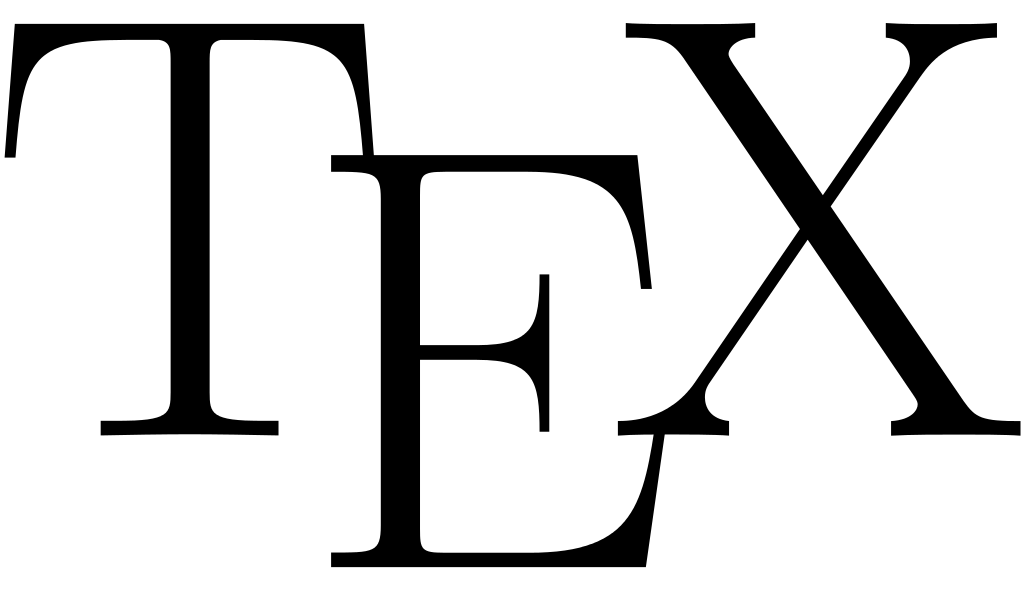
\includegraphics[height=16mm]{tex.png}
\end{center}
\end{frame}
%=========================
\begin{frame}[fragile]
\frametitle{\TeX{}}
Il est principalement conçu pour l'édition de documents techniques et est largement utilisé par les scientifiques, particulièrement en mathématiques, physique, bio-informatique, astronomie et informatique. Il est également extensible et permet notamment l'édition de documents plus complexes.
\TeX{} vient de τεχ, début du mot τέχνη, tékhnê (« art, science », en grec ancien), et se prononce /tɛx/2 ou /tɛk/, au choix.
\\[2mm]
Source : \url{https://fr.wikipedia.org/wiki/TeX}
\begin{center}
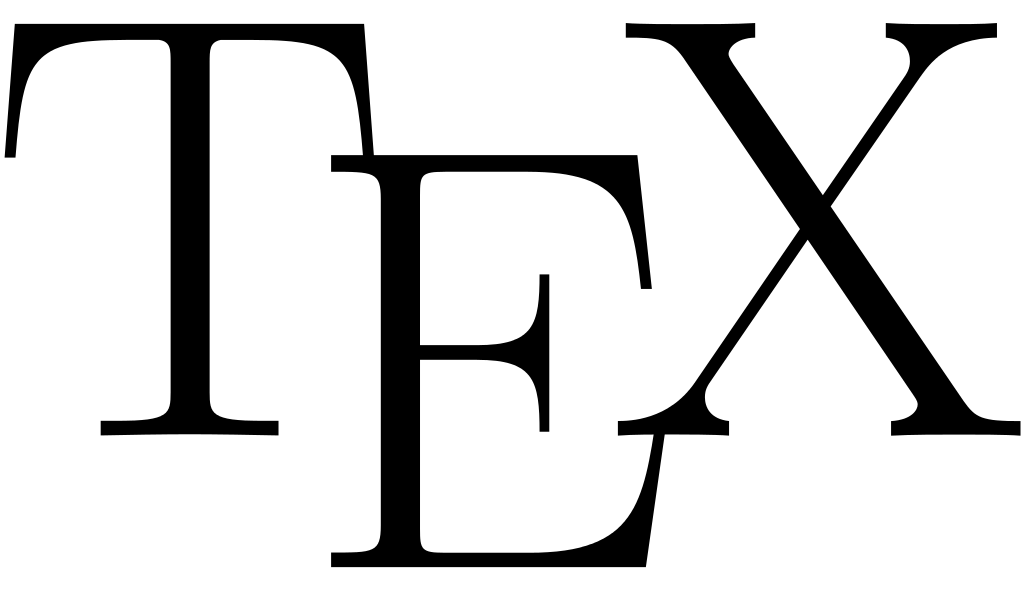
\includegraphics[height=16mm]{tex.png}
\end{center}
\end{frame}
%=========================
\begin{frame}[fragile]
\frametitle{\LaTeX{}}
\LaTeX{}  est un langage et un système de composition de documents. Il s'agit d'une collection de macrocommandes destinées à faciliter l'utilisation du « processeur de texte » \TeX{}.
\LaTeX{} permet de rédiger des documents dont la mise en page est réalisée automatiquement en se conformant du mieux possible à des normes typographiques. Une fonctionnalité distinctive de LaTeX est son mode mathématique, qui permet de composer des formules complexes.
\begin{center}

\includegraphics[height=16mm]{latex.png}
\end{center}
\end{frame}
%=========================
\begin{frame}[fragile]
\frametitle{\LaTeX{}}
\LaTeX{} est particulièrement utilisé dans les domaines techniques et scientifiques pour la production de documents de taille moyenne (tels que des articles) ou importante (thèses ou livres, par exemple). Néanmoins, il peut être employé pour générer des documents de types très variés (lettres ou transparents, par exemple). Enfin, de nombreux sites Internet — dont le texte est typiquement mis en forme par d’autres moyens — emploient un sous-ensemble de LaTeX pour composer notamment leurs formules mathématiques.
\\[2mm]
Source : \url{https://fr.wikipedia.org/wiki/LaTeX}
\begin{center}

\includegraphics[height=16mm]{latex.png}
\end{center}
\end{frame}
%=========================
\begin{frame}[fragile]
%
\begin{defn}
Quelque chose à lire\dots
\end{defn}
%
\begin{thm}
Quelque chose à lire\dots
\end{thm}
%
\begin{defn}
Quelque chose à lire\dots
\end{defn}
%
\begin{thm}
Quelque chose à lire\dots
\end{thm}
%
\begin{thm}[théorème]
Quelque chose à lire\dots
\end{thm}
%
% \begin{prop}[info]
% \scriptsize
% \lipsum[1]
% \end{prop}
%
% \begin{cor}
% Quelque chose à lire\dots
% \end{cor}
% %
% \begin{lem}
% Quelque chose à lire\dots
% \end{lem}
% %
% \begin{demo}
% Quelque chose à lire\dots
% \end{demo}
%
% \begin{theorem}
% Quelque chose à lire\dots
% \end{theorem}
% %
% \begin{proof}
% Quelque chose à lire\dots
% \end{proof}
% %
% \begin{corollary}
% Quelque chose à lire\dots
% \end{corollary}
% %
% \begin{lemma}
% Quelque chose à lire\dots
% \end{lemma}
% %
% \begin{example}
% Quelque chose à lire\dots
% \end{example}
% %
% \begin{alertblock}{Alert Block}
% Quelque chose à lire\dots
% \end{alertblock}
\end{frame}
%=========================
\begin{frame}[fragile]
\begin{lstlisting}[frame=tb]
let dfs g =
  let n = size g in
  let visited = Array.make n false in
  let rec dfs u =
    if not visited.(u) then (
      visited.(u) <- true;
      List.iter dfs (succ g u)
    );;
\end{lstlisting}
\end{frame}
%=========================
\begin{frame}[fragile]
\frametitle{Mathématiques}
\begin{align*}
\left( \int_{-\infty}^{+\infty} e^{-t^2} dt \right)^{2} & = 
\int_{0}^{2\pi} d\theta \left( \int_{0}^{+\infty} r^{2} e^{-r^2} dr \right)
\\
&= \sqrt{\pi}
\end{align*}
Suite de Fibonacci
\[
\begin{cases}
F_0 = 0 \quad F_1 = 1 \\
\forall n \in \N \quad F_{n+2} = F_{n+1} + F_{n}
\end{cases}
\]
\end{frame}
%=========================
\begin{frame}[fragile]
\begin{definition}[problème de l'arrêt en OCaml]
Le \emph{problème de l'arrêt} consiste à écrire une fonction OCaml :
\\
\centerline{\codec{halt: string -> string -> bool}}
prenant en entrées :
\begin{itemize}
\item une chaîne \codec{f} contenant le code source d'un programme OCaml,
\item une chaîne \codec{e} représentant des entrées pour le programme donné par \codec{f},
\end{itemize}
et qui, pour toutes chaînes \codec{f} et \codec{e}, termine en un temps fini en renvoyant \codec{true} si l'exécution du programme \codec{f} sur les entrées \codec{e} termine en temps fini, et \codec{false} sinon.
\end{definition}
\end{frame}
%=========================
\begin{frame}[fragile]
\begin{theorem}
Il n'existe pas de fonction OCaml résolvant le problème de l'arrêt.
\end{theorem}
%
\begin{demo}
Ce résultat se démontre par l'absurde, en supposant l'existence d'une fonction \codec{halt: string -> string -> bool} répondant à la spécification du problème de l'arrêt et en s'en servant pour construire un programme dont le comportement est contradictoire.

Supposons l'existence d'une telle fonction \codec{halt} et considérons alors la fonction \codec{weird} suivante.
\begin{lstlisting}
let weird f e =
  if halt f e then
    while true do print_string "ok" done;
\end{lstlisting}
\end{demo}
\end{frame}
%=========================
\begin{frame}[fragile]
\frametitle{Images}
\tikzstyle{every path} = [> = stealth', shorten > = 1pt, line width=1pt]
\tikzstyle{state} = [circle, fill=white, draw=black, text=black, minimum width=2mm, minimum size=6mm, inner sep=0pt, node distance=16mm, line width=1pt]
\tikzstyle{init} = [initial, initial text=]
\tikzstyle{term} = [accepting]
\begin{center}
\begin{tikzpicture}
\node[state, init, term] (0) {$0$};
\node[state, right of=0] (1) {$1$};
\node[state, right of=1] (2) {};
\node[state, right of=2, draw=white] (dots) {$\dots$};
\node[state, right of=dots] (n1) {};
\node[state, right of=n1] (n) {$n$};
\path[->]
(0) edge[bend left] node[above]{$a$} (1)
(1) edge[bend left] node[above]{$a$} (2)
    edge[bend left] node[below]{$b$} (0)
(2) edge[bend left] node[above]{$a$} (dots)
    edge[bend left] node[below]{$b$} (1)
(dots) edge[bend left] node[above]{$a$} (n1)
    edge[bend left] node[below]{$b$} (2)
(n1) edge[bend left] node[above]{$a$} (n)
    edge[bend left] node[below]{$b$} (dots)
(n) edge[bend left] node[below]{$b$} (n1)
;
\end{tikzpicture}
\end{center}
%
\begin{center}

\includegraphics[height=32mm]{img/aviary.png}
\end{center}
\end{frame}
%=========================
\end{document}


%=========================
\begin{frame}[fragile]
\end{frame}
